%----------------------------------------------------------------------------------------
%	PACKAGES AND OTHER DOCUMENT CONFIGURATIONS
%----------------------------------------------------------------------------------------

\documentclass[final]{beamer}

\usepackage[scale=1.24]{beamerposter} % Use the beamerposter package for laying out the poster

\usepackage{palatino}
\usepackage[most]{tcolorbox}
\usepackage{tikz-dependency}
\usepackage{tikz}
\usetikzlibrary{shapes,arrows}

\usetheme{confposter} % Use the confposter theme supplied with this template

\setbeamercolor{block title}{fg=ngreen,bg=white} % Colors of the block titles
\setbeamercolor{block body}{fg=black,bg=white} % Colors of the body of blocks
\setbeamercolor{block alerted title}{fg=white,bg=dblue!70} % Colors of the highlighted block titles
\setbeamercolor{block alerted body}{fg=black,bg=dblue!10} % Colors of the body of highlighted blocks
% Many more colors are available for use in beamerthemeconfposter.sty

\setbeamercolor{item}{fg=black}
\setbeamercolor{subitem}{fg=gray}


\newcommand\todo[1]{\textcolor{red}{\bf #1}}

%-----------------------------------------------------------
% Define the column widths and overall poster size
% To set effective sepwid, onecolwid and twocolwid values, first choose how many columns you want and how much separation you want between columns
% In this template, the separation width chosen is 0.024 of the paper width and a 4-column layout
% onecolwid should therefore be (1-(# of columns+1)*sepwid)/# of columns e.g. (1-(4+1)*0.024)/4 = 0.22
% Set twocolwid to be (2*onecolwid)+sepwid = 0.464
% Set threecolwid to be (3*onecolwid)+2*sepwid = 0.708

\newlength{\sepwid}
\newlength{\onecolwid}
\newlength{\twocolwid}
\newlength{\threecolwid}
\setlength{\paperwidth}{48in} % A0 width: 46.8in
\setlength{\paperheight}{36in} % A0 height: 33.1in
\setlength{\sepwid}{0.024\paperwidth} % Separation width (white space) between columns
\setlength{\onecolwid}{0.30\paperwidth} % Width of one column
\setlength{\twocolwid}{0.464\paperwidth} % Width of two columns
\setlength{\threecolwid}{0.708\paperwidth} % Width of three columns
\setlength{\topmargin}{-0.5in} % Reduce the top margin size
%-----------------------------------------------------------

\usepackage{graphicx}  % Required for including images

\usepackage{booktabs} % Top and bottom rules for tables

%----------------------------------------------------------------------------------------
%	TITLE SECTION 
%----------------------------------------------------------------------------------------

\title{Semantic Role Labeling for Process Recognition Questions} % Poster title

\author{Samuel Louvan$^+$,
		Chetan Naik$^+$,
		Veronica Lynn$^+$,
		Ankit Arun$^+$,
		Niranjan  Balasubramanian$^+$,
		Peter Clark$^*$} % Author(s)

\institute{$^+$Stony Brook University, 
    $^*$Allen Institute for AI\\
    \{slouvan, cnaik, velynn, aarun, niranjan\}@cs.stonybrook.edu,
    pclark@allenai.org} % Institution(s)

%----------------------------------------------------------------------------------------

\begin{document}

\addtobeamertemplate{block end}{}{\vspace*{2ex}} % White space under blocks
\addtobeamertemplate{block alerted end}{}{\vspace*{2ex}} % White space under highlighted (alert) blocks

\setlength{\belowcaptionskip}{2ex} % White space under figures
\setlength\belowdisplayshortskip{2ex} % White space under equations

\begin{frame}[t] % The whole poster is enclosed in one beamer frame

\begin{columns}[t] % The whole poster consists of three major columns, the second of which is split into two columns twice - the [t] option aligns each column's content to the top

\begin{column}{\sepwid}\end{column} % Empty spacer column

%----------------------------------------------------------------------------------------
%	COLUMN 1
%----------------------------------------------------------------------------------------

\begin{column}{\onecolwid} % The first column

%----------------------------------------------------------------------------------------
%	OBJECTIVES
%----------------------------------------------------------------------------------------
\begin{block}{Objective}
To develop a QA system that can answer a subset of 4\textsuperscript{th} grade questions involving recognizing instances of physical, biological, and other natural processes.\newline

The questions present a short description of an instance and multiple process names as the answer choices.
\vspace{15 mm}
%\begin{tcolorbox}[breakable,colback=gray!20!white,colframe=gray, boxrule=5pt, bottom=20pt, title=Example I/O]
\begin{tcolorbox}[breakable,colback=orange!50!yellow!20!white,colframe=orange!90!black!40, boxsep=10pt, bottom=20pt]

\textbf{Question:} As water vapor rises in the atmosphere, it cools and changes back to liquid. Tiny drops of liquid form clouds in this process called\\

\textbf{Answer Choices:}
\vspace{10mm}
\begin{itemize}
\setlength{\itemindent}{.5in}
\begin{minipage}{0.4\linewidth}
    \item condensation
    \item evaporation
\end{minipage}
\begin{minipage}{0.4\linewidth}
    \item precipitation
    \item run-off
\end{minipage}
\end{itemize}

\end{tcolorbox}

\end{block}


%----------------------------------------------------------------------------------------
%	INTRODUCTION
%----------------------------------------------------------------------------------------

\begin{block}{Approach}

This work explores a knowledge-driven approach to answering such questions. 
\begin{itemize}
	\item We represent processes using a light-weight semantic role based representation.
	\item We answer a question by assessing how well the roles of the instance in the question align with the roles of the candidate answer processes.
\end{itemize}

\end{block}

%------------------------------------------------

\begin{figure}
%\includegraphics[width=0.8\linewidth]{qa_sys.pdf}
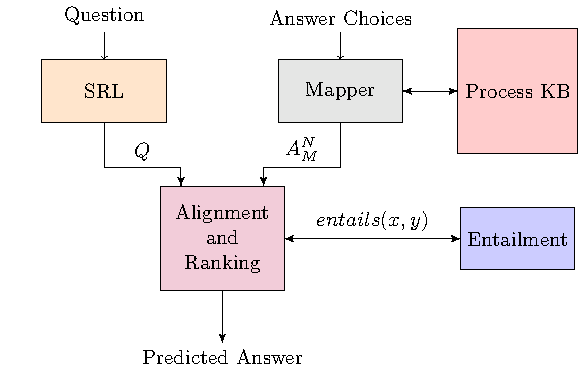
\includegraphics[width=0.8\linewidth]{diagram.pdf}
\end{figure}

%----------------------------------------------------------------------------------------

\end{column} % End of the first column

\begin{column}{\sepwid}\end{column} % Empty spacer column

%----------------------------------------------------------------------------------------
%	COLUMN 2
%----------------------------------------------------------------------------------------

\begin{column}{\onecolwid}

%----------------------------------------------------------------------------------------
%	Representing Processes via Semantic Roles
%----------------------------------------------------------------------------------------

\begin{block}{Representing Processes via Semantic Roles}

The 4\textsuperscript{th} grade level questions do not require deep knowledge about the sub-events of processes or their sequential order. The required knowledge can be expressed via semantic roles. 
Accordingly we design a simple representation that encodes information about each process via the following roles:
\begin{enumerate}
\item {\em Input} -- This role captures the main input to the process or the object undergoing the process.
\item {\em Result} -- The artifact that results from the process or the change that results from the process.
\item {\em Trigger} -- The main action, expressed as a verb or its nominalization, indicating the occurrence of the process.
\item {\em Enabler} -- The artifact, condition or action that enables the process to happen.
\end{enumerate}


\begin{figure}
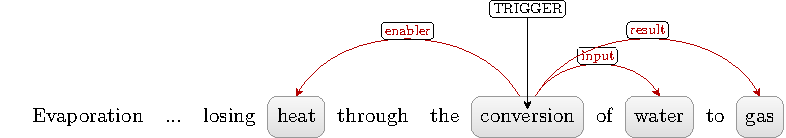
\includegraphics[width=\linewidth]{srl.pdf}
\end{figure}

\begin{itemize}
	\item We use MATE  SRL system \cite{bjorkelund2009multilingual} for role labeling.
	\item To account for the limited amount of training data, we explored distant supervision, and domain adaptation \cite{daume2009frustratingly}.
\end{itemize}



\end{block}

%----------------------------------------------------------------------------------------
%	Question Answering Using Semantic Roles
%----------------------------------------------------------------------------------------

\begin{block}{Question Answering Using Semantic Roles}

We score each candidate answer process based on how well the roles of the instance described in the question align with the roles of the process. We use the following procedure to answer questions:\\
\begin{itemize}
\item Identify the roles in the question statement $(Q)$. 
\item Collect the roles for all the answer processes $(A_{1..M}^{1..N})$ from the Knowledge Base.
\emph{($M$-- \# of answer choices, $N$-- \# of frames)}\\
\item For every QA frame pair, compute an alignment score by checking for the textual entailment of the corresponding roles.
$$alignment(Q, A_m^n) = \sum_{role_i \in R} entails(role_i(A_m^n), role_i(Q))$$
where, $R =$\{Input, Result, Enabler, Trigger\}. $entails(x, y)$ is computed as a textual entailment score that reflects how well the text $x$ entails text $y$ or the other way around. 
\item Compute the mean of the top 5 frame alignment scores for each process and return the top scoring process as the answer.
\end{itemize}

\end{block}

%----------------------------------------------------------------------------------------

\end{column} % End of the second column

\begin{column}{\sepwid}\end{column} % Empty spacer column

%----------------------------------------------------------------------------------------
%	COLUMN 3
%----------------------------------------------------------------------------------------

\begin{column}{\onecolwid} % The third column

%----------------------------------------------------------------------------------------
%	RESULTS
%----------------------------------------------------------------------------------------

\begin{block}{Results}

\begin{table}[htdp]
\begin{center}
\begin{tabular}{l p{0.01\linewidth} c p{0.01\linewidth} c p{0.01\linewidth} c}
\hline
\textbf{Method}			&& 	\textbf{Precision}	&&	\textbf{Recall}	&&	\textbf{F1}\\
\hline
Standard			&& 	0.4323	&& 	0.3325	&&	0.3758\\
Per Process		&&	0.4225	&& 	0.2556	&& 	0.3185\\
Distant Supervision 	&& 	{\bf 0.5614}	&& 	0.2642	&& 	0.3594 \\
Dom. Adaptation	&& 	0.4386	&& 	{\bf 0.3351}	&& 	{\bf 0.3799}\\
\hline
\end{tabular}
\end{center}
\caption{Semantic Role Labeling Performance}
\label{tab:srl-results}
\end{table}

\begin{table}[htdp]
\begin{center}
\begin{tabular}{ l p{0.1\linewidth} c }
\hline
\textbf{Method} & & \textbf{Accuracy}\\
\hline
BOW &&  63.12\\
Manual SRL & & 67.38\\
BOW+Manual SRL & & {\bf 70.92}\\
\hline
Standard	& & {\bf 55.32}\\
Per Process & & 46.80 \\
Domain Adaptation & & {\bf 55.32}\\
Distant Supervision & & 51.77\\
\hline
BOW + Standard  & & {\bf 65.24}\\
\hline
\end{tabular}
\caption{Question Answering Performance}
\label{tab:qa-results}
\end{center}
\vspace{-3ex}
\end{table}

\end{block}


%----------------------------------------------------------------------------------------
%	ERROR ANALYSIS
%----------------------------------------------------------------------------------------

\begin{block}{Error Analysis}

{\bf Automatic SRL Failures}
\begin{itemize}
	\item Issues that arise out of data sparsity
	\item Gap between verb-based role and our customized process-based role
\end{itemize}
\vspace{5mm}
{\bf QA Failures}
\begin{itemize}
	\item Knowledge Representation Issues (37\%)
	\item Entailment Issues (32\%)
	\item Scoring Issues (31\%) 
\end{itemize}

\end{block}
\vspace{-0.5in}
%----------------------------------------------------------------------------------------
%	REFERENCES
%----------------------------------------------------------------------------------------

\begin{block}{References}

\nocite{*} % Insert publications even if they are not cited in the poster
\small{\bibliographystyle{unsrt}
\bibliography{mybib}\vspace{0in}}

\end{block}

%----------------------------------------------------------------------------------------
%	ACKNOWLEDGEMENTS
%----------------------------------------------------------------------------------------

\setbeamercolor{block title}{fg=orange,bg=white} % Change the block title color

\begin{block}{Acknowledgements}

\small{\rmfamily{This work is funded in part by Fulbright PhD Fellowship and by the Allen Institute for Artificial Intelligence. The findings and conclusions expressed herein are those of the authors alone.}} \\

\end{block}

%----------------------------------------------------------------------------------------

\end{column} % End of the third column

\end{columns} % End of all the columns in the poster

\end{frame} % End of the enclosing frame

\end{document}
